\documentclass[hyperref={pdfpagelabels=false}]{beamer}
\usepackage{lmodern}
\usepackage{pgf}
\usepackage{tikz}
\usetikzlibrary{arrows}
\usetikzlibrary{automata}
\usetikzlibrary{shapes.geometric}
\usepackage{subcaption}
\usetheme{Berlin}
\definecolor{UniRed}{RGB}{255,0,0}
\definecolor{UniWhite}{RGB}{255,255,255}
\setbeamercolor{eecks} {bg=UniRed, fg=UniWhite}
\title{\textsc{RoboSoccer} Project Plan}  
\author[Hofbauer, Jiang, Meyer, Schmidt, Wirnshofer]{
  Markus~Hofbauer \and
  He~Jiang \and
  Kevin~Meyer \and
  Benedikt~Schmidt \and
  Florian~Wirnshofer
}
\institute
{
	Technische Universit\"at M\"unchen, Germany
}
\date{\today} 
\begin{document}
\begin{frame}
\titlepage
\end{frame}

\begin{frame}
	\frametitle{Implementation}
	\begin{figure}
		\centering
		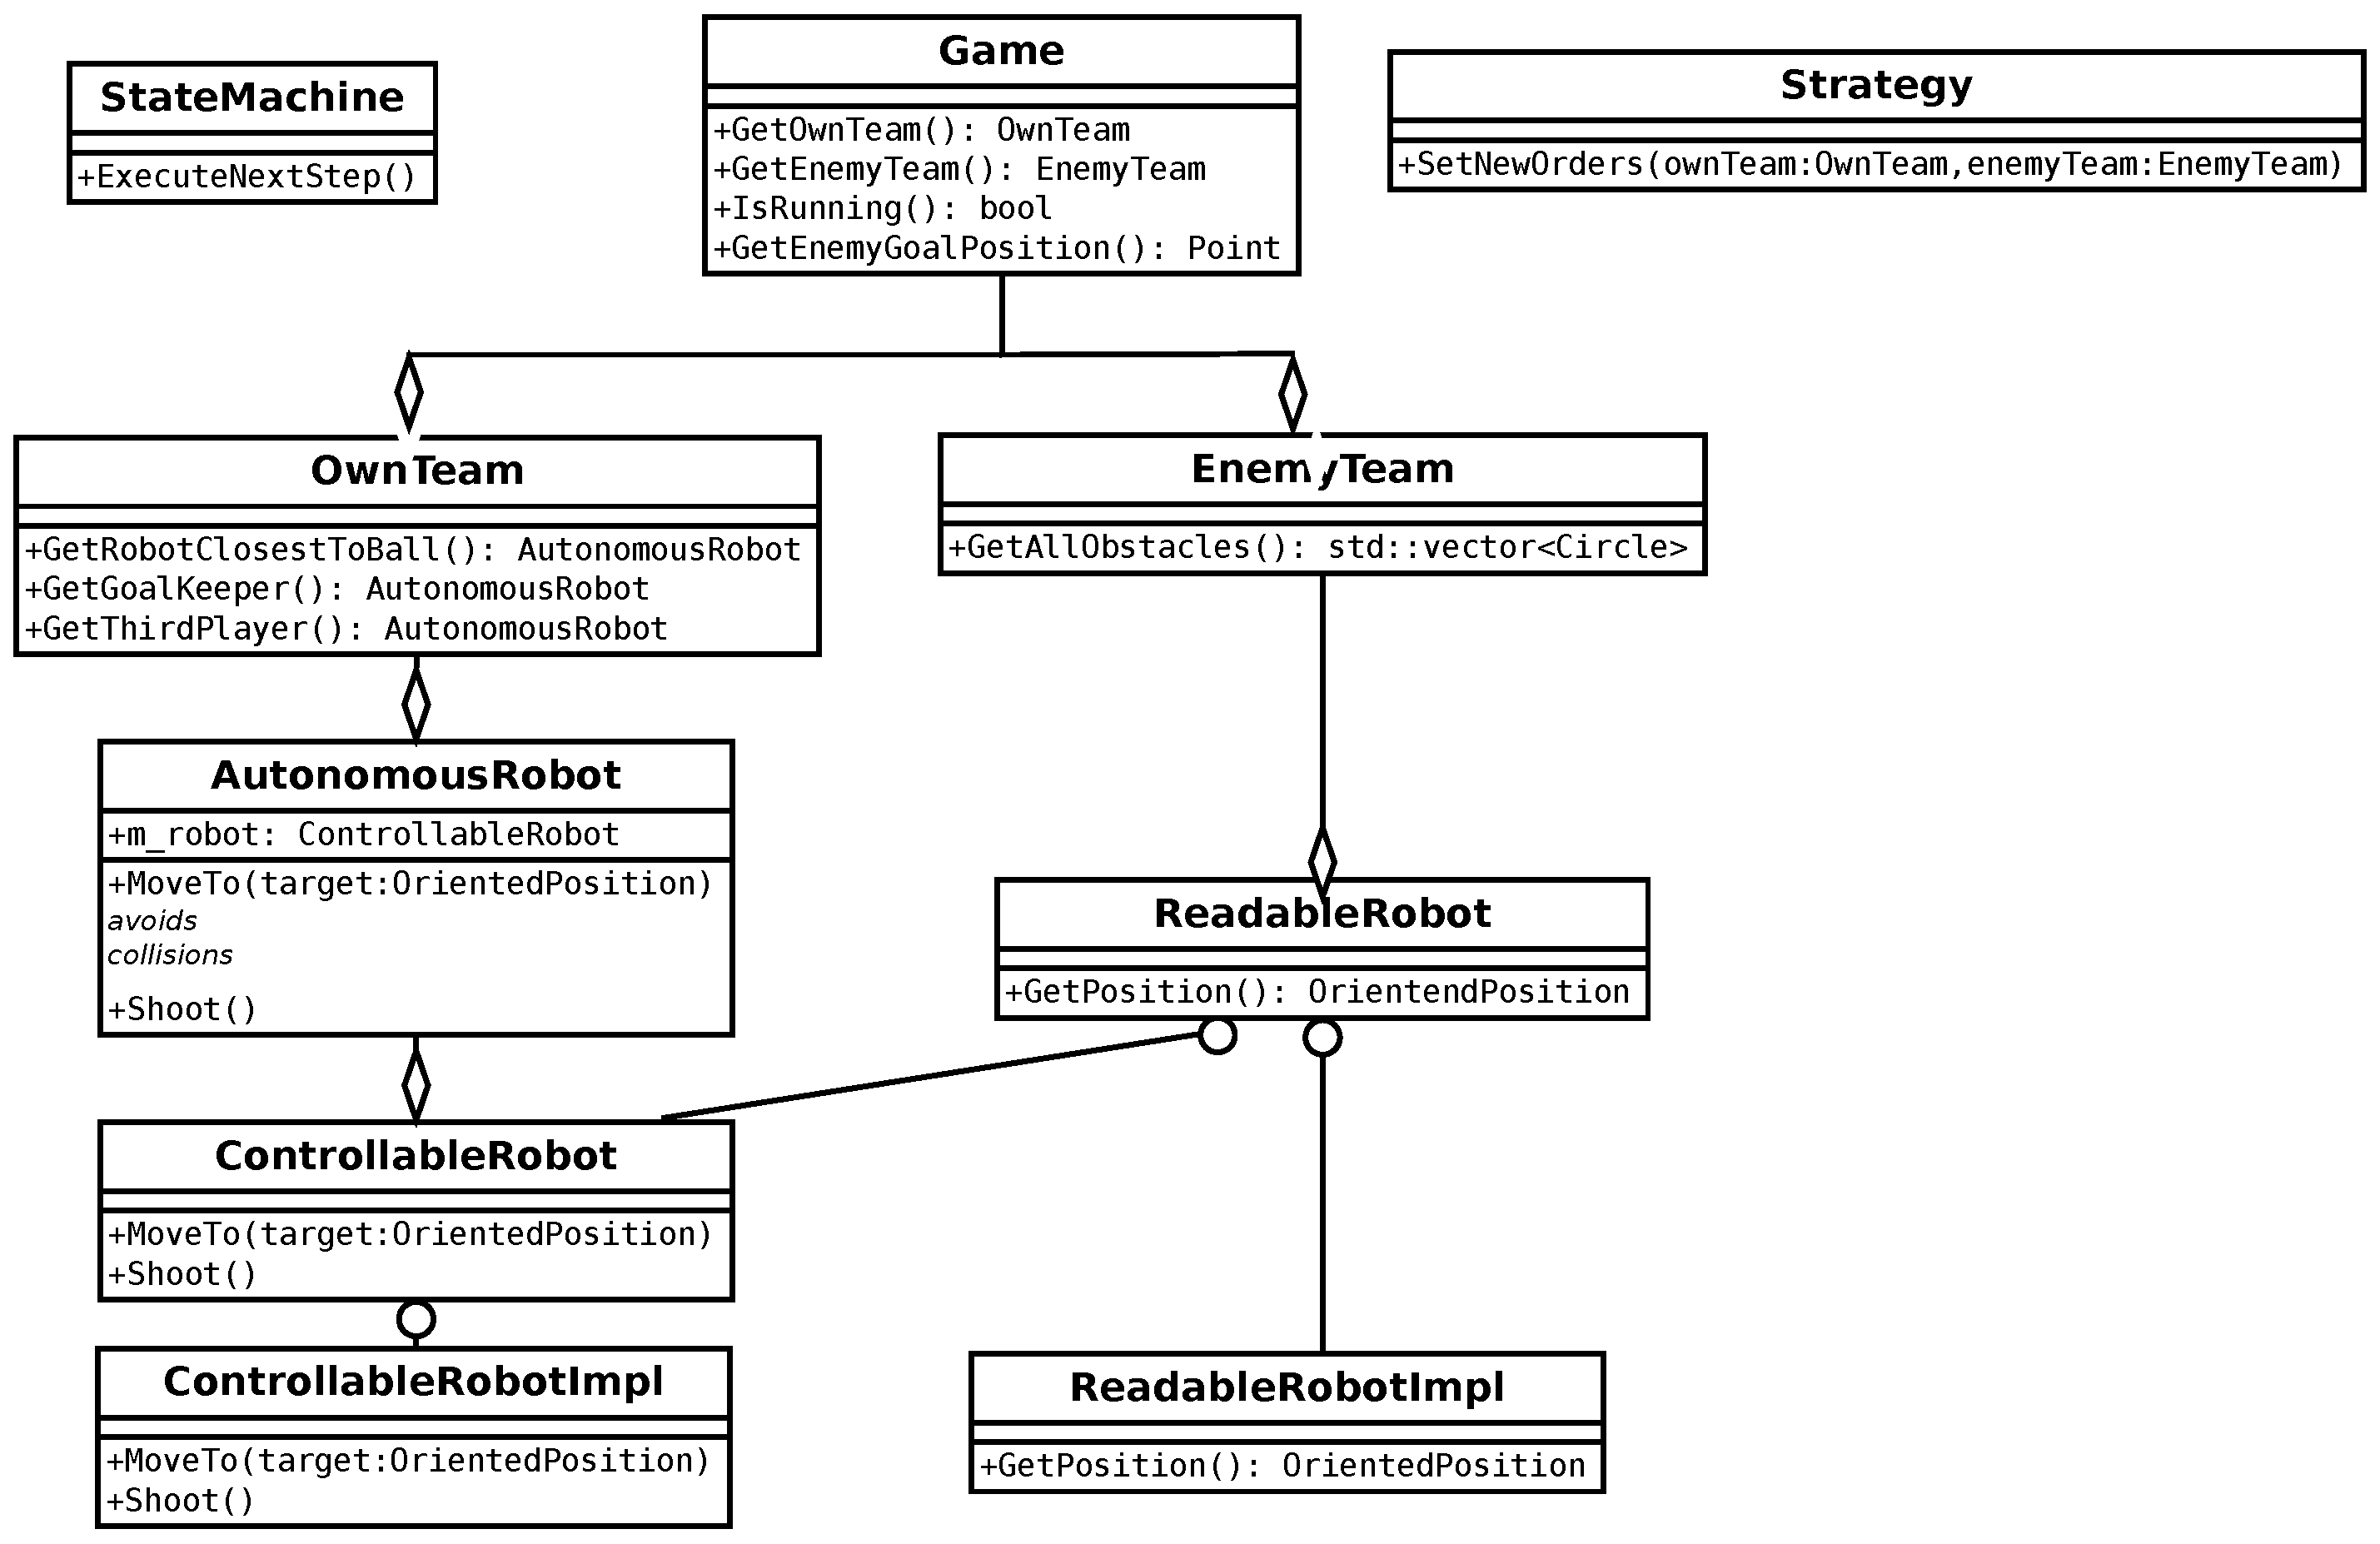
\includegraphics[width = 0.9\textwidth]{architecture}
	\end{figure}
\end{frame}

\begin{frame}
	\frametitle{State Machine}
	\fontsize{6pt}{7.2}\selectfont
	
	\begin{columns}
		\column{.8\textwidth}
		\begin{center}
			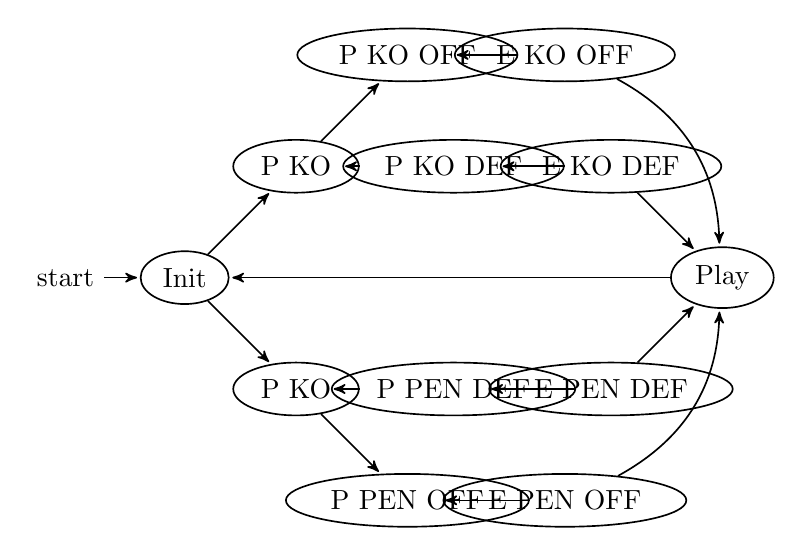
\begin{tikzpicture}[->,>=stealth',shorten >=1pt,auto,node distance=2cm,
			                    semithick]
			  \tikzstyle{every state}=[draw=none,text=black]
			  \tikzset{elliptic state/.style={draw,ellipse}}
			
			  \node[initial,elliptic state] (init)                    {Init};
			  \node[elliptic state]         (prepareKickOff) [above right of=init] {P KO};
			  \node[elliptic state]         (prepareKickOffOffensive) [above right of=prepareKickOff] {P KO OFF};
			  \node[elliptic state]         (executeKickOffOffensive) [right of=prepareKickOffOffensive] {E KO OFF};
			  \node[elliptic state]         (prepareKickOffDefensive) [right of=prepareKickOff]       {P KO DEF};
			  \node[elliptic state]         (executeKickOffDefensive) [right of=prepareKickOffDefensive]       {E KO DEF};
			  \node[elliptic state]         (preparePenalty) [below right of=init] {P KO};
			  \node[elliptic state]         (preparePenaltyOffensive) [below right of=preparePenalty] {P PEN OFF};
			  \node[elliptic state]         (executePenaltyOffensive) [right of=preparePenaltyOffensive] {E PEN OFF};
			  \node[elliptic state]         (preparePenaltyDefensive) [right of=preparePenalty]       {P PEN DEF};
			  \node[elliptic state]         (executePenaltyDefensive) [right of=preparePenaltyDefensive]       {E PEN DEF};
			  \node[elliptic state]         (play) [below right of=executeKickOffDefensive]       {Play};
			
			  \path (init) 
			  			edge (prepareKickOff)
			  			edge (preparePenalty)
			        (prepareKickOff) 
			        	edge (prepareKickOffOffensive)
			            edge (prepareKickOffDefensive)
			        (prepareKickOffOffensive)
			        	edge (executeKickOffOffensive)
			        (prepareKickOffDefensive)
			        	edge (executeKickOffDefensive)
			        (executeKickOffOffensive)
			        	edge [bend left] (play)
			        (executeKickOffDefensive)
			        	edge (play)
			        (preparePenalty) 
			        	edge (preparePenaltyOffensive)
			            edge (preparePenaltyDefensive)
			        (preparePenaltyOffensive)
			        	edge (executePenaltyOffensive)
			        (preparePenaltyDefensive)
			        	edge (executePenaltyDefensive)
			        (executePenaltyOffensive)
			        	edge [bend right] (play)
			        (executePenaltyDefensive)
			        	edge (play)
			        (play)
			        	edge (init);
			\end{tikzpicture}
		\end{center}
		\column{.1\textwidth}
		\begin{center}
			\begin{tabular}{cc}
				P & prepare \\
				KO & kick-off \\
				OFF & offensive \\
				DEF & defensive \\
				E & execute \\
				PEN & penalty
			\end{tabular}
		\end{center}
	\end{columns}
\end{frame}

\begin{frame}
	\frametitle{Progress}
	UPDATED GANTT CHART MISSING
\end{frame}

\end{document}

